\writer{Alber, Javier, Marius, Ruxandra}

As the previous chapter has shown, our implementation is very complex and a variety of situations have been
taken into account. Due to our multi-agent, conflict solving and heuristics-based approach, as expected, the
program works very well on some types of maps,  but there are, of course, cases where it doesn't perform that
well. The most relevant cases will be analyzed further on.

\subsection{Single Agent}

The first thing we will analyse is how the system performs in a single-agent, deterministic environment.
Because of the heuristics we use, the solutions we are finding are near-optimal. Even though this is very good
for small maps, as the agent performs a really small number of actions, on large maps with a big number of
boxes, it takes a long time to compute the solution. However, due to the low-level optimizations done in our
implementation code, the search and expansions are extremely fast.

Another case in which the solution is very difficult to find is when there is a large number of boxes that
have to be moved out of the way for the agent to achieve its goal. This happens because the agent does not
know at the beginning how to move the boxes in a free space as it only has goals related to delivering a box
to a goal cell or clearing a path. In the future, a possible solution that we could use to solve this issue is
to add another type of goal for partially cleaning important and tricky parts of the map, which could be
assigned to each agent at the beginning.

Regarding the evaluation of the how the agents are being assigned the \textit{correct} goal, we have observed
that the defined heuristic was correctly guiding the agent to the optimal solution in all of our tests.

Figure~\ref{fig:goalplanneraresults}, presents an example of a solution produced by the system. Blue cells indicate boxes, while yellow cells indicate goal cells. Numbers indicate the order in which they were solved. It can be observed that the agent correctly identified the non-blocking goals as well as the ones that were closer to them (this is, the distance to the box, and from the box to the goal).

\begin{figure}[htb]
\begin{center}
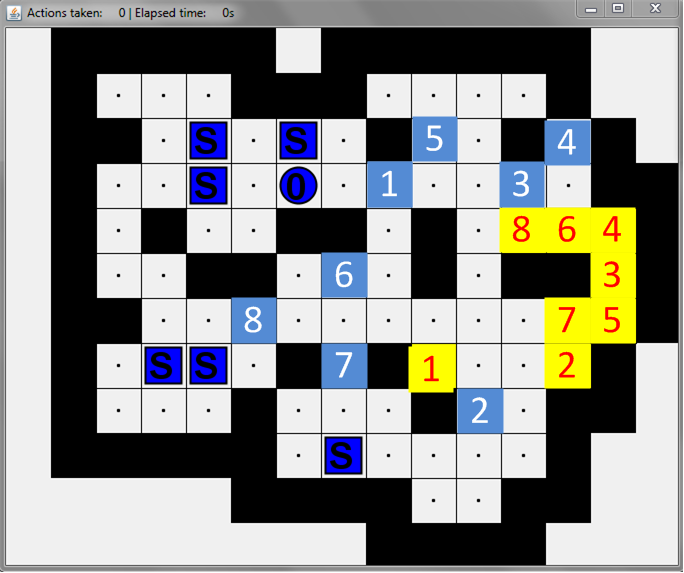
\includegraphics[width=0.4\textwidth]{figures/example_goal_planner}
\caption{Evaluation of the Goal Planner Heuristic}
\label{fig:goalplanneraresults}
\end{center}
\end{figure}

A side-effect of trying to find optimal solutions is that more time is needed in order to come up with the
solution. This is not very noticeable on small maps, but on larger maps, with more boxes, the time difference
can be easily observed.

After testing on various levels, we can say that the presented solution solves most of the Hanoi-like maps.
This is done with the special heuristic described in Section~\ref{sec:heuristics}..

Figure ~\ref{fig:results_hanoi} presents how the agent 0 is solving the map mentioned above, Figure
\ref{fig:heuristics2}.

\begin{figure}[htb]
\begin{center}
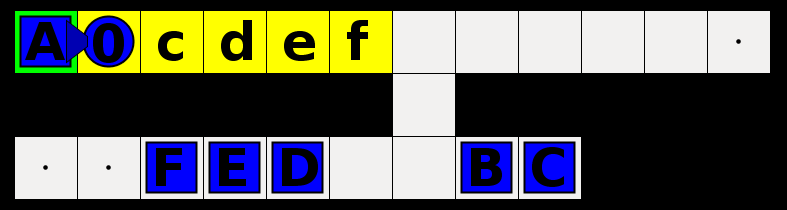
\includegraphics[width=0.5\textwidth]{figures/results_hanoi.png}
\caption{Agent 0 solving of the map in Figure \ref{fig:heuristics2}}
\label{fig:results_hanoi}
\end{center}
\end{figure}

An important aspect that should be mentioned when talking about heuristics is the pre-analysis of the map.
Because we can’t perform a complete analysis of the state at each step of the expansion as it would have been
very computationally demanding, we try to base our heuristic on information that can be computed before
starting the actual processing.

\subsection{Multi-agent} %FOMA / POMA
An observation which needs to be made is that the approach chosen was pure multi-agent planning, so each agent
creates its own plan, and only needs special communication with the central entity when conflicts are
detected. In some of the maps, multibody planning could have worked better. However, at least in theory,
multibody planning would not scale very well for large maps and a big number of agents. On the other hand, our
solution also had some problems with scaling for a large number of boxes/goals as the used heuristics did not
take all the parameters into account.

The result of multi-agent system in complex levels is not very good, because the central entity makes real
merging for each agent's plan, instead of just delaying one of the agents that are in conflict. While merging
works well when there is a conflict between only two agents as it finds the optimal merging in a reasonable
amount of time, it fails to work in cases where there are more than two agents and their actions can’t be
merged only by delaying and there is a need for extra-actions to be performed. Even though this solution is
time-consuming, it provides a solution that is more similar to a real-case scenario.

In POMA levels, the agents are capable of detecting the unknown objects that block their path and can recover
from this situation without any problems. Figure ~\ref{fig:poma_step1} shows how the agent wants to complete
its goal but finds an unknown object that stops it. Once the agent has updated its beliefs, it generates
another plan and tries again to complete its goal. Figure \ref{fig:poma_step2} presents how after some
interactions the agent manages to find the correct path.

\begin{figure}[htb]
\begin{center}
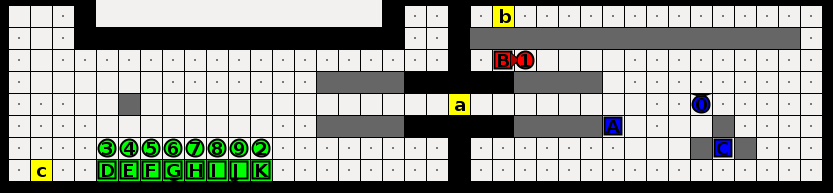
\includegraphics[width=0.8\textwidth]{figures/POMA_step1}
\caption{The agent 1 finds an unknown object in its path.}
\label{fig:poma_step1}
\end{center}

\end{figure}
\begin{figure}[htb]
\begin{center}
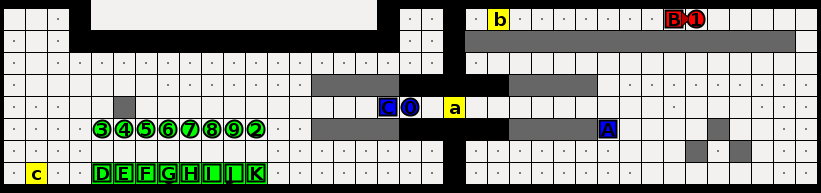
\includegraphics[width=0.8\textwidth]{figures/POMA_step2}
\caption{Agent 1 finally success in finding a path without unknown objects.}
\label{fig:poma_step2}
\end{center}
\end{figure}

The presented system has been tested in a competition against the projects developed by other students. The
results show that the system is able to handle single agent maps with good results, being the group resolving
with fewest actions three of the thirteen maps.

However, multiagent environments did not present the same performance and results were not as good as
expected. While we were able to find more optimal solutions by merging plans of the agents and replanning if
necessary, the fact that we opted for a multiagent system instead of multibody had a huge impact on the
results in some scenarios.